\documentclass[../main.tex]{subfiles}

\begin{document}

\subsubsection*{1\hfill}
Construct a state diagram for a DFA (``deterministic finite-state automaton'') that recognizes the set of all bit strings that contain an odd number of $0$-bits and end with two $1$-bits.

\solution
\begin{center}
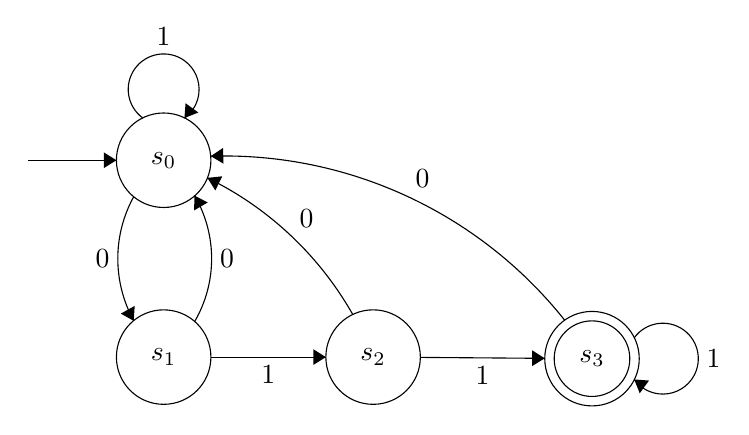
\begin{tikzpicture}[scale=0.2]
\tikzstyle{every node}+=[inner sep=0pt]
\draw [black] (13,-20.2) circle (3);
\draw (13,-20.2) node {$s_0$};
\draw [black] (13,-32.7) circle (3);
\draw (13,-32.7) node {$s_1$};
\draw [black] (26.3,-32.7) circle (3);
\draw (26.3,-32.7) node {$s_2$};
\draw [black] (40.2,-32.8) circle (3);
\draw (40.2,-32.8) node {$s_3$};
\draw [black] (40.2,-32.8) circle (2.4);
\draw [black] (4.4,-20.2) -- (10,-20.2);
\fill [black] (10,-20.2) -- (9.2,-19.7) -- (9.2,-20.7);
\draw [black] (11.105,-30.396) arc (-151.08865:-208.91135:8.162);
\fill [black] (11.1,-30.4) -- (11.16,-29.45) -- (10.28,-29.94);
\draw (9.59,-26.45) node [left] {$0$};
\draw [black] (11.677,-17.52) arc (234:-54:2.25);
\draw (13,-12.95) node [above] {$1$};
\fill [black] (14.32,-17.52) -- (15.2,-17.17) -- (14.39,-16.58);
\draw [black] (14.962,-22.446) arc (30.30024:-30.30024:7.936);
\fill [black] (14.96,-22.45) -- (14.93,-23.39) -- (15.8,-22.88);
\draw (16.55,-26.45) node [right] {$0$};
\draw [black] (16,-32.7) -- (23.3,-32.7);
\fill [black] (23.3,-32.7) -- (22.5,-32.2) -- (22.5,-33.2);
\draw (19.65,-33.2) node [below] {$1$};
\draw [black] (29.3,-32.72) -- (37.2,-32.78);
\fill [black] (37.2,-32.78) -- (36.4,-32.27) -- (36.4,-33.27);
\draw (33.25,-33.26) node [below] {$1$};
\draw [black] (42.88,-31.477) arc (144:-144:2.25);
\draw (47.45,-32.8) node [right] {$1$};
\fill [black] (42.88,-34.12) -- (43.23,-35) -- (43.82,-34.19);
\draw [black] (15.78,-21.322) arc (63.99832:29.55377:21.387);
\fill [black] (15.78,-21.32) -- (16.28,-22.12) -- (16.72,-21.22);
\draw (22.07,-24.48) node [above] {$0$};
\draw [black] (15.988,-19.943) arc (91.79923:38.4903:27.609);
\fill [black] (15.99,-19.94) -- (16.8,-20.42) -- (16.77,-19.42);
\draw (29.44,-21.98) node [above] {$0$};
\end{tikzpicture}
\end{center}
\end{document}
